\section{Theory}
% 3 Theory
% 3.1 Mechanics of Bolted Connection Loading

% Figure 4: Bolted Joint Diagram

% The schematic above shows what a typical bolted connection looks like. The key forces in the
% above diagram are the preload, Fi, and the external load, P. This connection can be viewed as an
% analogy to the spring system seen below.

% Figure 5: Spring Analogy

% When the spring system is at rest, the inside spring, kb is tensioned while the outside springs, km
% is compressed. The inside spring can be thought of as the bolt, and the outside as the joined
% member, with the spring constants equivalent to the stiffnesses of the materials. The preload is
% created when the nut on the bolt is tightened. The deflection of the bolt and the member are given
% by the equations below.

% 7

% δb =
% Fi
% kb
% (1)

% δm =
% Fi
% km
% (2)

% When the external load, P, is applied to the joint a change in the deformation of the bolt and the
% reduction of compression in the joined members. This change in deformation can be calculated
% using the equations:

% ∆δb =
% Pb
% kb
% (3)

% ∆δm =
% Pm
% km
% (4)

% Assuming that no separation occurs, the deformation in the member and the bolt are equivalent,
% shown by the relation below:

% Pb
% kb
% =
% Pm
% km
% (5)

% Taking the external load as a product of the load on the bolt and the member gives:

% P = Pm + Pb (6)
% Rearranging the above expression with Equation (5) yields:

% Pb =
% kbP
% kb+km
% (7)

% Pm =
% kmP
% kb+km
% (8)

% These equations give the changes in the external loading in both the bolt and the member. Their
% total loads are given by:

% Fb = Fi + Pb (9)
% Fm = Fi + Pm (10)

% 8

% 3.2 Bridge Equations
% The voltage reading from the bridge, Eo can be expressed using the input voltage, Ein, Gauge
% factor, Kg, gain, G, and strain, ε.

% Eo =
% KgEinGε
% 4
% (11)

% Since the output voltage is the given reading from the MTS machine and strain gauge, this
% equation will be rearranged to solve for strain (see Appendix A). As a way of calibrating the
% bolted connection, the equivalent strain simulated by the shunt resistor is given by:

% εeq =
% Rg
% NaKg(Rs+Rg)
% (12)

% 3.3 The Stress-Strain Relationship
% A key factor for analyzing the strength of bolted members is the relation between stress and
% strain. The Young’s Modulus (or Modulus of Elasticity), a constant denoted as Eb, shows this
% proportionality.

% σ = Ebε (13)

% The force exerted on the bolt can be shown using the applied stress and the strained cross-
% sectional area.

% Fb = Asσ (14)

% 3.4 Bolt Stiffness
% A bolt can be separated to into various section with differing cross-sectional areas to get an
% overall value for the stiffness of the bolt. Let’s say there is i sections through the bolt, each
% stiffness can be evaluated as:

% ki =
% AiEb
% Li
% (15)

% Then for the stiffness of the entire bolt:
% 1
% kb
% = ∑
% 1
% ki
% n
% i=1
% (16)

% 9

% 3.5 Member Stiffness
% The stiffness of the overall member is tougher to evaluate without some key assumptions. The
% figure below shows the diagram of a member in compression

% Figure 5: Analysis of the compression of members in a bolted connection

% With a gasket, the member stiffness can be evaluated using the same idea presented in Equation
% 16, considering the gasket as a section of the bolt. However, since the material is much softer in
% the gasket, it tends to dominate the equation for member stiffness. Without a gasket, the load
% spreads out between the head of the bolt and the nut, and is harder to evaluate. By assuming that
% the angle of stress distribution is 45o, a simplified expression for the bolt stiffness can found.

% km =
% πEbd
% 2ln {5[
% L+0.5d
% L+2.5d
% ]}
% (17)

% 3.6 Torque Requirement for Preloading
% Referring back to the preload force discussed earlier, this is often applied as torque to tighten the
% nut on the end of the bolt. This relationship is given as:

% T = Fid{[
% dm
% 2d
% ][
% tanλ+μ sec α
% 1 − μ tan λ sec α

% ] + 0.625 μc
% (18)

% The expression in the braces can be simplified to K, known as the torque constant. Equation 18
% then becomes:

% T = KdFi
% (19)

% 10
% K is typically within the ranges of 0.10 (lubricated threads) and 0.20 (lubricated thread)
% 3.7 Bolt Preload for Static Loading
% Preloading the bolt is meant to prevent the jointed member from separating and the bolt from
% yielding. Using Equations (7) and (9), the total load on the bolt can be given by:

% Fb = Fi + CP (20)

% Where the constant C is defined as:
% C =
% kb
% kb+km
% (21)

% 3.8 Bolt Preload for Dynamic Loading
% Cyclic loading cycles are used to vary the load on a bolt over time. The two parameters often
% analyzed from these trials are the mean and alternating stresses.

% σm =
% σmax + σmin
% 2

% (22)

% σa =
% σmax− σmin
% 2

% (23)

\subsection{Mechanics of Bolted Connections Loading}
The typical bolted connection is shown in Figure \ref{fig:bolted_joint_diagram}. The key forces in the above diagram are the preload, $F_i$, and the external load, $P$. This connection can be viewed as an analogy to the spring system seen in Figure \ref{fig:spring_analogy}.
\begin{figure}[h]
    \centering
    \begin{subfigure}[b]{0.4\textwidth}
        \centering
        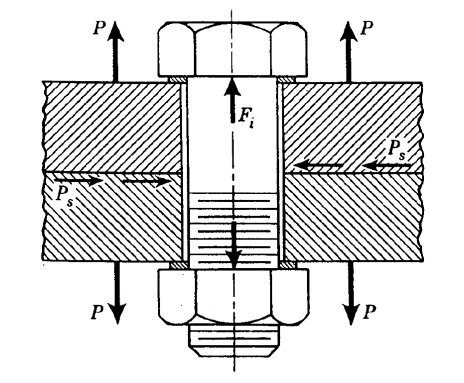
\includegraphics[width=0.5\textwidth]{Sections/Figures/bolted connection force diagram.png}
        \caption{}
        \label{fig:bolted_joint_diagram}
    \end{subfigure}
    \begin{subfigure}[b]{0.4\textwidth}
        \centering
        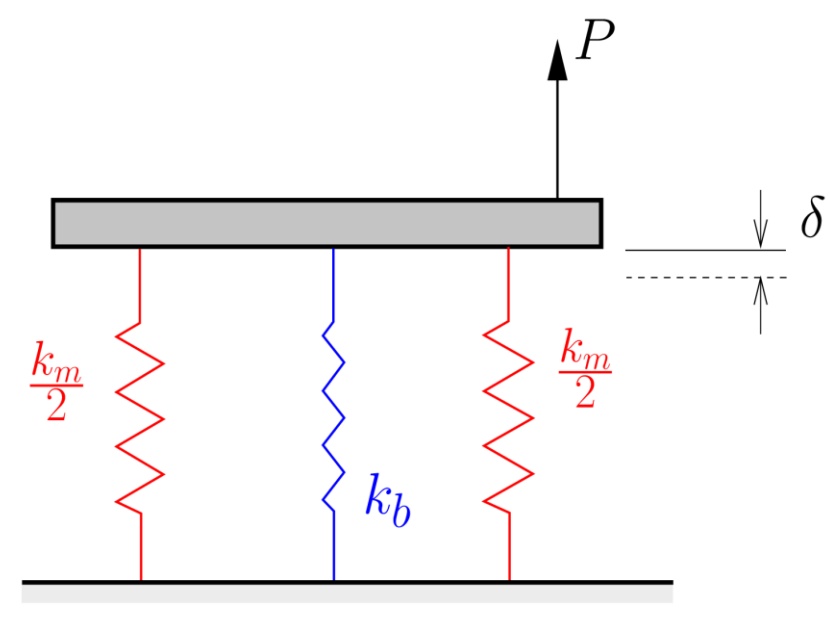
\includegraphics[width=0.5\textwidth]{Sections/Figures/spring analogy.png}
        \caption{}
        \label{fig:spring_analogy}
    \end{subfigure}
    \caption{a) Bolted Joint Diagram with Preload and External Load, b) Spring Analogy}
\end{figure}
By Hooke's law, the deflection of the bolt and the member are given by the equations below:
\begin{align}
    \delta_b &= \frac{F_i}{k_b} \label{eq:delta_b} \\
    \delta_m &= \frac{F_i}{k_m} \label{eq:delta_m}
\end{align}
When the external load, $P$, is applied to the joint, a change in the deformation of the bolt and the reduction of compression in the joined members occurs. Similar to deflection, the change in deformation can be calculated using the equations:
\begin{align}
    \Delta \delta_b &= \frac{P_b}{k_b} \label{eq:delta_delta_b} \\
    \Delta \delta_m &= \frac{P_m}{k_m} \label{eq:delta_delta_m}
\end{align}
If the members are not separated, the deformation in the member and the bolt are equivalent, shown by the relation below:
\begin{equation}
    \frac{P_b}{k_b} = \frac{P_m}{k_m} \label{eq:delta_no_separation}
\end{equation}
The total load on the bolt and the member must equal the sum of the change in load of the bolt, $P_b$, and the member, $P_m$, 
\begin{align*}
    P &= P_m + P_b 
\end{align*}
Using (\ref{eq:delta_no_separation}), the change in load of the bolt and the member can be expressed as:
\begin{align}
    P_b &= \frac{k_bP}{k_b+k_m} \label{eq:P_b} \\
    P_m &= \frac{k_mP}{k_b+k_m} \label{eq:P_m}
\end{align}
Similarly, the total loads on the bolt and the member are given by:
\begin{align}
    F_b &= F_i + P_b \label{eq:F_b} \\
    F_m &= F_i + P_m \label{eq:F_m}
\end{align}

\subsection{Quarters Bridge Equations}
The instrumented bolt uses a Wheatstone quarter bridge to measure strain. The voltage reading from the bridge, $V_o$, can be expressed using the input voltage, $V_{in}$, gauge factor, $K_g$, gain, $G$, and strain, $\varepsilon$.
\begin{equation}
    \varepsilon = \frac{4V_o}{K_gV_{in}G} \label{eq:strain_bridge}
\end{equation}

\subsection{Stress-Strain Relationship}
By Hooke's law, the stress-strain relationship is given by:
\begin{equation}
    \sigma = E_b\varepsilon \label{eq:stress_strain}
\end{equation}
Since stress is force per unit area, 
\begin{equation}
    F_b = A_s\sigma \label{eq:force_area}
\end{equation}

\subsection{Member Stiffness}
Members in a bolted connection can be viewed as a series of springs. Equivalent stiffness for this system is given by:
\begin{align}
    \frac{1}{k_m} &= \sum_{i=1}^{n} \frac{1}{k_i} \label{eq:member_stiffness_series} \\
\end{align}
where $k_i$ is the stiffness of the $i$th section of the member. 

For members with a gasket, loading can be estimated by assuming the load spreads at a fixed 45$^\circ$ angle. The compression of each element is then divided into infinitesimally small annular elements. It can be shown that the stiffness for two identical members bolted together is given by:
\begin{figure}[h]
    \centering
    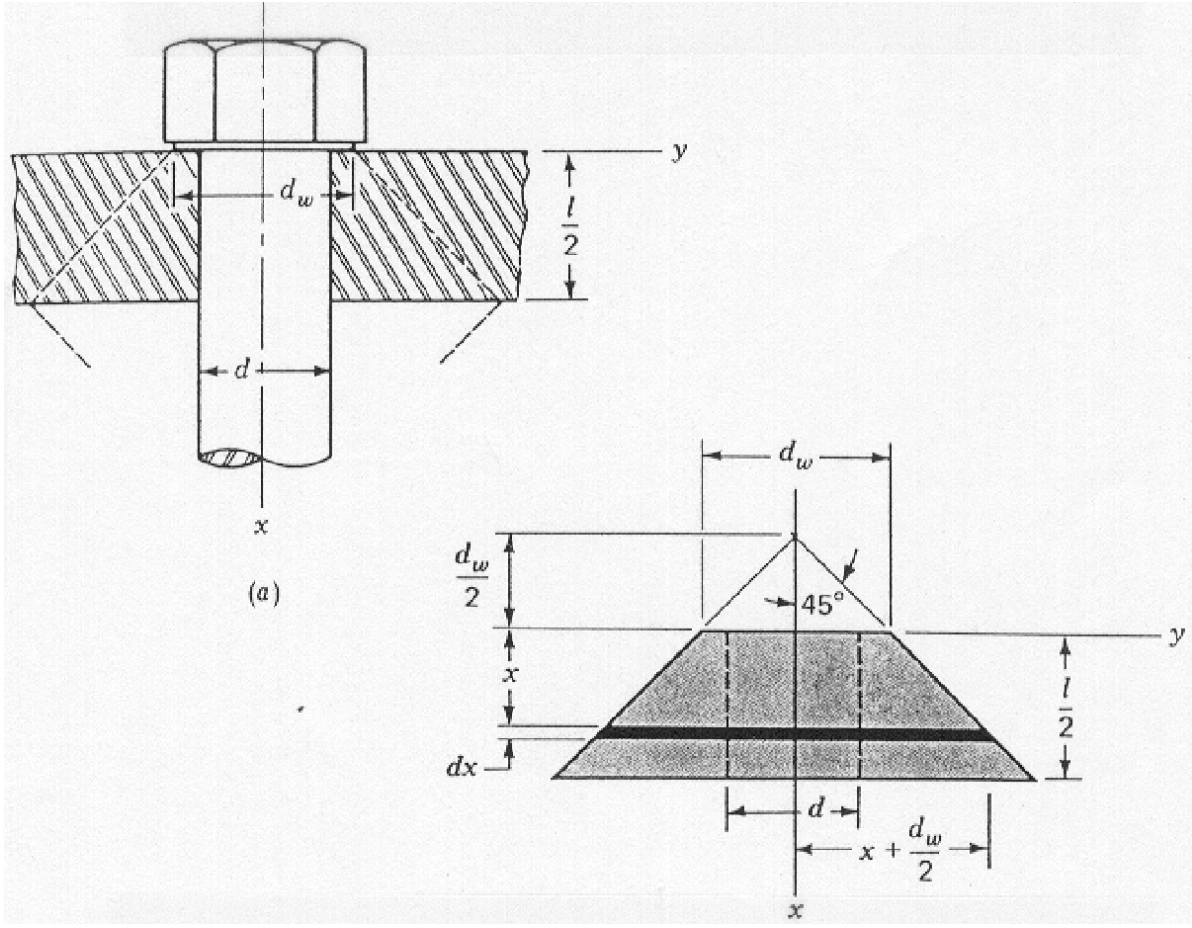
\includegraphics[width=0.5\textwidth]{Sections/Figures/bolted connection gasket analysis.png}
    \caption{Analysis of the compression of members in a bolted connection}
    \label{fig:bolted_connection_gasket_analysis}
\end{figure}
\begin{equation}
    k_m = \frac{\pi E_b d}{2\ln\left(\frac{5(L+0.5d)}{L+2.5d}\right)} \label{eq:member_stiffness}
\end{equation}

\subsection{Torque Requirement for Preloading}
From basic screw-thread theory, the torque required to preload a bolt is given by:
\begin{align*}
    T &= \frac{F_i d}{2}\left[\frac{L + \pi \mu d_m \sec\alpha}{\pi d_m - \mu L \sec\alpha}\right] 
\end{align*}
it can be shown that 
\begin{align}
    T &= F_i d \left[ \left(\frac{d_m}{2d}\right)\left(\frac{\tan\lambda + \mu \sec\alpha}{1 - \mu \tan\lambda \sec\alpha}\right) + 0.625\mu_c \right]  \nonumber \\
    &= KdF_i \label{eq:torque_constant}
\end{align}

\subsection{Bolt Preload for Static Loading}
Preloading the bolt is meant to prevent the jointed member from separating and the bolt from yielding. Using Equations (\ref{eq:P_b}) and (\ref{eq:F_b}), the total load on the bolt can be given by:
\begin{equation}
    F_b = F_i + CP \label{eq:total_load_bolt}
\end{equation}
where the constant $C$ is defined as:
\begin{equation}
    C = \frac{k_b}{k_b+k_m} \label{eq:constant_C}
\end{equation}
at the point of joint separation, $F_b = P$. Rearranging (\ref{eq:total_load_bolt}) gives:
\begin{equation}
    F_i = P(1-C) \label{eq:joint_separation}
\end{equation}
To avoid yielding, a safety factor is introduced, $N$. Rearranging (\ref{eq:total_load_bolt}) gives:
\begin{equation}
    F_i = \frac{A_t \sigma_{y}}{N} - CP \label{eq:yielding}
\end{equation}

\subsection{Bolt Preload for Dynamic Loading}
Cyclic loading cycles are used to vary the load on a bolt over time. The two parameters often analyzed from these trials are the mean and alternating stresses.
\begin{align}
    \sigma_m &= \frac{F_{\text{max}} + F_{\text{min}}}{2A_s} \label{eq:mean_stress} \\
    \sigma_a &= \frac{F_{\text{max}} - F_{\text{min}}}{2A_s} \label{eq:alternating_stress}
\end{align}
The modified Goodman criteria states:
\begin{align*}
    \frac{\sigma_a}{\sigma_e} + \frac{\sigma_m}{\sigma_{ut}} &= 1
\end{align*}
where $\sigma_e$ is the endurance limit, and $\sigma_{ut}$ is the ultimate tensile strength. It can be shown the follow holds,
\begin{align*}
    F_i &= A_s \sigma_{ut} - \frac{NCP}{2} \left[\frac{\sigma_{ut}}{\sigma_e} - 1\right]
\end{align*}